\section{Motivation for Dynamic Coding}\label{sec:parsec_motivation}
%\subsubsection{Motivation}
Bank conflicts are most likely to occur when regions of shared memory are localized to certain memory regions. Multi-core systems often generate memory access requests to overlapping memory regions. By dynamically coding certain memory locales, the proposed memory system aims to resolve the bank conflicts which occur during periods of heavy memory access in multi-core systems.

\begin{figure}[htbp]
		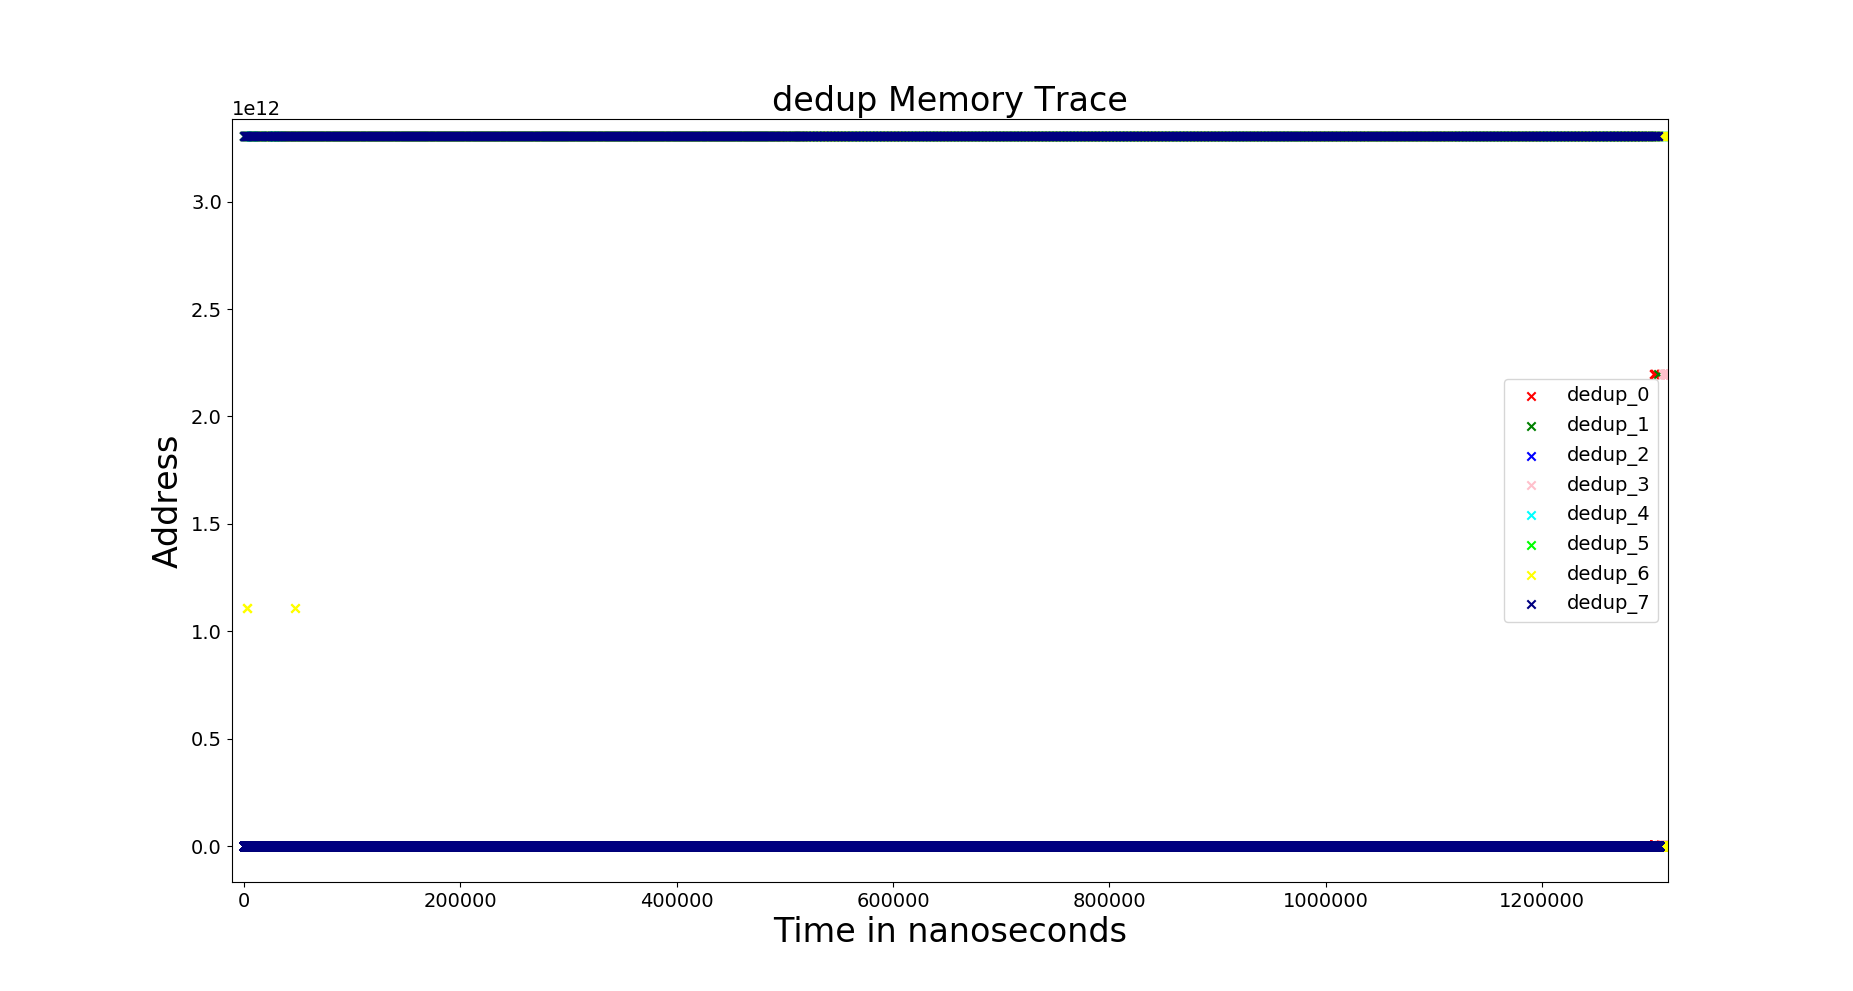
\includegraphics[width=\linewidth]{fig/dedup_whole.png}
		\caption{\it{Memory Access from the Dedup PARSEC benchmark. This trace was generated using 8 cores.}}
		\label{fig:dedup_whole}
\end{figure}

\begin{figure}[htbp]
		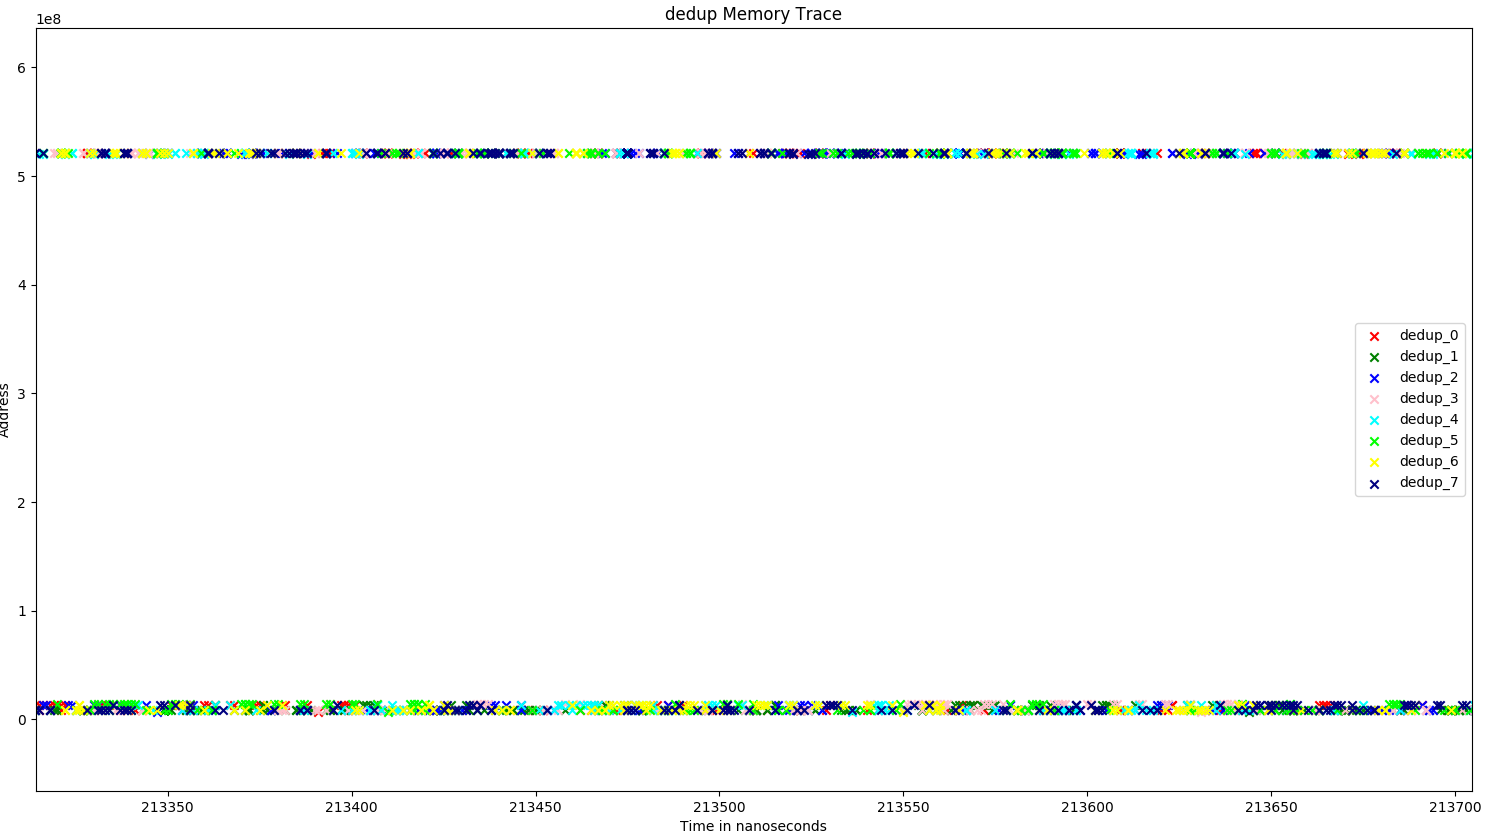
\includegraphics[width=\linewidth]{fig/dedup_dense.png}
		\caption{\it{Memory Access from the Dedup PARSEC benchmark demonstrating the density of memory accesses}}
		\label{fig:dedup_dense}
\end{figure}

An examination of the memory trace from one of the PARSEC benchmarks illustrates a scenario where dynamic coding works well. Figure~\ref{fig:dedup_whole} shows the memory trace of a simulation of an 8-core system running the dedup PARSEC benchmark. The y-axis shows the address accessed by the cores. The x-axis shows the access time in nanoseconds. This plot shows that most of the accesses from various cores are primarily located in the lower memory band. Greater than 95\% of all memory accesses are in this band. Figure~\ref{fig:dedup_dense} magnifies this band and reveals that the lower band is composed of two sub-bands of roughly equal density. In a scenario where the dynamic coder can choose to encode two memory blocks it would detect that nearly all memory access are localized to the primary memory bands, so only those regions would be encoded.


Figure~\ref{fig:dedup_dense} shows that the dedup benchmark contains very dense memory utilization. Across all processors, there is an average of $1.11$ ns between accesses per core. This implies an average of $2.22$ cycles between memory access requests per $2$ Ghz processor. Crucially, the most heavily used memory regions are stationary with respect to time for all PARSEC benchmarks. 

Figure~\ref{fig:dedup_whole} shows an entire dedup memory trace. There are two major bands clearly visible in this image, and the bands stay in the same memory regions for the entirety of the trace. Figure~\ref{fig:dedup_dense} is a magnified view of the bottom band. This figure reveals that the bottom band is composed of two sub-bands which are also stationary with respect to time. The structure of the dedup the memory trace is representative for all the PARSEC benchmarks. It is also clear from this image that the memory regions utilized by all of the processors overlap sufficiently to create bank conflicts.

